%
\documentclass{aip-cp}

\usepackage[numbers]{natbib}
\usepackage{rotating}
\usepackage{graphicx}
\usepackage{lmodern}
\usepackage[T1]{fontenc}
\usepackage{wasysym}

% Document starts
\begin{document}

% Title portion
\title{MICROCONTROLLERS ESP32 STM32}

\author[aff1]{D.A. Nikiforov}
\eaddress{ndorofei@gmail.com}
\author[aff2]{A.A. Bugaev}
\eaddress{dihlo1@yandex.ru}


\affil[aff1]{SVFU.}
\affil[aff2]{SVFU.}

\maketitle

\begin{abstract}
ESP32 is a series of low-cost, low-power system on a chip microcontrollers with integrated Wi-Fi and dual-mode Bluetooth. The ESP32 series employs a Tensilica Xtensa LX6 microprocessor in both dual-core and single-core variations and includes in-built antenna switches, RF balun, power amplifier, low-noise receive amplifier, filters, and power-management modules. ESP32 is created and developed by Espressif Systems, a Shanghai-based Chinese company, and is manufactured by TSMC using their 40 nm process.It is a successor to the ESP8266 microcontroller.
STM32 is a family of 32-bit microcontroller integrated circuits by STMicroelectronics. The STM32 chips are grouped into related series that are based around the same 32-bit ARM processor core, such as the Cortex-M7F, Cortex-M4F, Cortex-M3, Cortex-M0+, or Cortex-M0. Internally, each microcontroller consists of the processor core, static RAM memory, flash memory, debugging interface, and various peripherals.

\end{abstract}

% Head 1
\section{INTRODUCTION}
The STM32 is a family of microcontroller ICs based on the 32-bit RISC ARM Cortex-M7F, Cortex-M4F, Cortex-M3, Cortex-M0+, and Cortex-M0 cores.[1] STMicroelectronics licenses the ARM Processor IP from ARM Holdings. The ARM core designs have numerous configurable options, and ST chooses the individual configuration to use for each design. ST attaches their own peripherals to the core before converting the design into a silicon die. The following tables summarize the STM32 microcontroller families.
ESP32 is a series of low-cost, low-power system on a chip microcontrollers with integrated Wi-Fi and dual-mode Bluetooth. The ESP32 series employs a Tensilica Xtensa LX6 microprocessor in both dual-core and single-core variations and includes in-built antenna switches, RF balun, power amplifier, low-noise receive amplifier, filters, and power-management modules. ESP32 is created and developed by Espressif Systems, a Shanghai-based Chinese company, and is manufactured by TSMC using their 40 nm process.[2] It is a successor to the ESP8266 microcontroller.

%Head 2
\section{History}

The STM32 is the third ARM family by STMicroelectronics. It follows their earlier STR9 family based on the ARM9E core,[7] and STR7 family based on the ARM7TDMI core.[8] The following is the history of how the STM32 family has evolved.

In October 2006, STMicroelectronics (ST) announced that it licensed the ARM Cortex-M3 core.[9]
In June 2007, ST announced the STM32 F1-series based on the ARM Cortex-M3.[10]
In November 2007, ST announced the low-cost "STM32-PerformanceStick" development kit in partner with Hitex.[11]
In October 2009, ST announced that new ARM chips would be built using the 90 nm process.[12]
In April 2010, ST announced the STM32 L1-series chips.[13]
In September 2010, ST announced the STM32VLDISCOVERY board.[14]
In November 2010, ST announced the STM32 F2-series chips based on the ARM Cortex-M3 core, and future development of chips based on the ARM Cortex-M4 and ARM Cortex-M3 cores.[15]
In February 2011, ST announced the STM32L-DISCOVERY board.[16]
In March 2011, ST announced the expansion of their STM32 L1-series chips with flash densities of 256 KB and 384 KB.[17]
In September 2011, ST announced the STM32 F4-series chips based on the ARM Cortex-M4F core and STM32F4DISCOVERY board.[18]
In February 2012, ST announced the STM32 F0-series chips based on the ARM Cortex-M0 core.[19]
In May 2012, ST announced the STM32F0DISCOVERY board.[20]
In June 2012, ST announced the STM32 F3-series chips based on the ARM Cortex-M4F core.[21]
In September 2012, ST announced full-production of STM32 F3-series chips and STM32F3DISCOVERY board. The STM32 F050-series will also be available in a TSSOP20 package.[22]
In January 2013, ST announced full Java support for STM32 F2 and F4-series chips.[23]
In February 2013, ST announced STM32 Embedded Coder support for MATLAB and Simulink.[24]
In February 2013, ST announced the STM32 F4x9-series chips.[25]
In April 2013, ST announced the STM32 F401-series chips.[26]
In July 2013, ST announced the STM32 F030-series chips. The STM32 F030-series will also be available in a TSSOP20 package.[27]
In September 2013, ST announced the STM32F401C-DISCO and STM32F429I-DISCO boards.[28]
In October 2013, ST announced the STM32F0308DISCOVERY board.[29]
In December 2013, ST announced that it is joining the mbed project.[30]
In January 2014, ST announced the STM32 F0x2-series chips, STM32F072B-DISCO board, and STM32072B-EVAL board.[31]
In February 2014, ST announced the STM32 L0-series chips based on the ARM Cortex-M0+ core.[32]
In February 2014, ST announced multiple STM32 Nucleo boards with Arduino headers and mbed IDE.[33]
In February 2014, ST announced the release of free STM32Cube software tool with graphical configurator and C code generator.[34]
In April 2014, ST announced the STM32F30x chips are now available in full production. A new NUCLEO-F302R8 board was also announced.[35]
In September 2014, ST announced the STM32 F7 series, the first chips based on the Cortex-M7F core.[36]
In October 2016, ST announced the STM32H7 series based on the ARM Cortex-M7F core. The device runs at 400 MHz and is produced using 40 nm technology.



The long wave propagation in the ocean is governed by the so-called 
shallow-water differential equations:

\[
H_t + (uH)_x + (vH)_y = 0,
\]
\begin{equation}
\label{eq1}
u_t + uu_x + vu_y + gH_x = gD_x ,
\end{equation}
\[
v_t + uv_x + vv_y + gH_y = gD_y ,
\]

\noindent
where \textit{H(x, y, t) = h(x, y, t) + D(x, y, t), h} is the water surface displacement, D is depth, u(x, y, t) and v(x, y, 
t) are velocity components along the axes x and y, g is acceleration of 
gravity. The initial conditions: still water at all grid points except a 
tsunami source where a surface displacement is not equal to zero. From the 
shallow-water equations it follows that the tsunami propagation velocity 
does not depend on its length and is expressed by the so-called Lagrange 
formula [2]

\begin{equation}
\label{eq2}
c = \sqrt {g(D + \eta )} .
\end{equation}

This formula plays the key role for the long-wave (tsunami) kinematics. From 
the shallow-water equations the ratio between the running wave height and 
the water flow velocity can be derived. The horizontal flow velocity depends 
on the wave amplitude and water depth

\begin{equation}
\label{eq3}
u = \eta \sqrt {\frac{g}{D}} \quad .
\end{equation}

These relations between tsunami wave parameters are used in the algorithm 
proposed.

The numerical algorithm is based on splitting the difference scheme that 
approximates equations (\ref{eq1}) by spatial directions. A finite difference 
algorithm based on the splitting method has been developed in [2]. To solve 
the shallow wave equations, the splitting method reduces the numerical 
solution with two spatial variables to the solution of two one-dimensional 
equations. It makes possible to use effective finite difference schemes 
developed for one-dimensional problems. Moreover, this method permits one to 
set boundary conditions for a finite difference boundary value problem using 
a characteristic line method. The criterion of stability for the MOST 
algorithm can be written down as 

\begin{equation}
\label{eq4}
\Delta t \le \frac{\Delta x} { \sqrt{gH}} .
\end{equation}

Here $\Delta t$ and $\Delta x$ are the time and the grid steps, respectively. 
This condition requires setting a smaller time step if a computational 
domain contains deep-water areas. For example, if a deep-water trench with a 
depth of 9,000 m is included into the area with 1,000~m resolution 
computational grid, then we must use a 3 sec (or less) time step for the 
stability of computation. At one time step, a tsunami wave must advance a 
distance less than one spatial grid step. In the case of tsunami occurrence, 
a deep-water detector can give the passing tsunami wave parameters 15-20 
minutes after the main shock of a tsunamigenic earthquake. Then a few 
minutes are necessary to obtain the first estimates of the tsunami source 
parameters and its center, in particular, the location of the center (the 
locality of a maximum vertical displacement of the water surface) and a 
value of a maximum vertical elevation. This information allows us to begin 
the numerical calculation of a direct problem of tsunami propagation from 
the source, actually, to the coastline (up to depths of 5-10 m). However, 
for obtaining results of the tsunami propagation, be more reliable 
(distribution of tsunami wave heights in a shelf zone), rather a small step 
of a computational grid (about tens meters) is necessary. If we simulate the 
tsunami propagation in the whole area including both a source zone and sites 
of the coast, we are interested in, using this small spatial grid step, then 
because of the stability condition we will be compelled to carry out 
calculation with a small time step. This will bring about a significant 
increase in the time of numerical calculation that is inadmissible in 
real-time calculations. Therefore it is necessary to carry out such 
calculations with the use of the computational grids whose spatial step 
decreases when approaching the coast.


\section{A MODEL OF ELLIPSOIDAL TSUNAMI SOURCE}
A standard MOST software package uses as an initial water surface elevation 
that is equal to the ocean bottom displacement obtained as a result of 
numerical modeling of the elastic-plastic problem with seismic source with 
specified parameters. In this case, it is not easy to set the initial water 
surface displacement with a specified amplitude at the desired locality. 
However, sometimes it is needed to study the ratio between the initial wave 
height and wave parameters near the coast. In this case it is necessary to 
carry out a number of numerical experiments with specified initial 
parameters. For this purpose two algorithms can be implemented into the MOST 
software package. The first subroutine defines the initial water surface 
displacement having the ellipsoidal shape. Inside this ellipse, the surface 
elevation is expressed by the formula

\begin{equation}
\label{eq5}
H(i,j) = \left( {1 + \cos (\pi \cdot \arg (i,j))} \right) \cdot H_0 ,
\end{equation}

\noindent
where $H_{0}$ is half the water surface displacement at the central point 
($i_{0}$, $j_{0})$ of the ellipse. The parameter \textit{arg(i,j)} gives the ratio between the 
distance to the ellipse center and the distance to the ellipse border in 
this direction

\begin{equation}
\label{eq6}
\arg (i,j) = \left( {\frac{(i - i_0 ) \cdot \cos (\beta ) + (j - j_0 ) \cdot 
\sin (\beta )}{r_1 }} \right)^2 + \left( {\frac{(j - j_0 ) \cdot \cos (\beta 
) - (i - i_0 ) \cdot \sin (\beta )}{r_2 }} \right)^2.
\end{equation}

Here $r_{1}$, $r_{2}$ are the ellipse axis length and \textit{$\beta $} is the long axis 
azimuth. Figure 1 shows the shape of the 2 meters height ellipsoidal source 
with the axes ratio equal to 2 and the water height distribution along the 
ellipse axis.

\begin{figure}[ht]
  \centerline{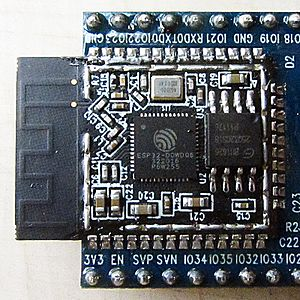
\includegraphics[width=250pt]{art/Fig_01.png}}
  \caption{STM 32}
\end{figure}

Thus, this subroutine gives the possibility of the numerical simulation of 
the tsunami waves generated by such a kind of sources with a specified 
location and an initial height. Another way to generate a wave with given 
parameters (an amplitude and a wavelength or a period) is to use boundary 
conditions. For example, let at the initial instant of time in the whole 
computational domain the water surface elevation and flow velocity 
components be equal to zero. Then at all the grid points along one boundary 
(for example, left) the following free boundary conditions are fulfilled 
during a limited time period:

\begin{equation}
\label{eq7}
\eta = \frac{\eta _0 }{2}\left( {1 - \cos \left( {\frac{2\pi \cdot t}{T}} 
\right)} \right),
\quad
u = \eta \sqrt {\frac{g}{D}} ,
\end{equation}

\noindent
where \textit{$\eta $}$_{0}$ is a wave height and $T$ is its period, $g$ is the gravity 
acceleration, $D$ is the depth. As a result, the flat tsunami wave having the 
amplitude \textit{$\eta $}$_{0}$ and the period T will propagate from this left boundary 
inside the computational domain.

\section{MULTI-GRID COMPUTATIONS OF THE TSUNAMI WAVE PROPAGATION}

We propose the algorithm, which consists in a consecutive calculation of the 
tsunami wave propagation in several computational domains, where each 
subsequent computational area is a subarea to the previous one, but with a 
smaller spatial step. And initially in these subareas there is no tsunami 
source (the initial vertical water surface displacement). Information on 
parameters of a wave is transferred to each subsequent subarea through 
boundary conditions, thus these data are interpolated along the boundary on 
a smaller computational grid. 

\subsection{Nested Computational Domains}
Digital bathymetry sets were taken or 
developed using different sources. The first stage of the numerical 
simulation uses the whole-Pacific gridded bathymetry developed by Smith and 
Sandwell [5], which is now used by the NOAA for the trans-pacific tsunami 
modeling. The limits of this computational domain are shown in Figure 2.

\begin{figure}[h]
  \centerline{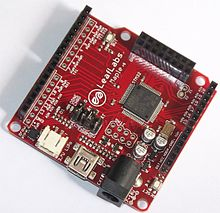
\includegraphics[width=250pt]{art/Fig_02.png}}
  \caption{ ESP 32}
\end{figure}

Resolution of this digital bathymetry is varying from 4 arc minutes (about 
8,000 m) at the equator to 2 arc minutes (approx. 4,000 m) closer to the 
polar areas. The geographic coverage of these data (area B0) is from 
120$^{o}$ E to 68$^{o}$ W and from 73.96$^{o}$ S up to 62$^{o}$ N.

For further stages of the modeling, the area of the Pacific Ocean adjacent 
to the northwest of the island of Honshu (Japan) is chosen. The gridded 
digital bathymetry for the numerical modeling was developed using 500 m 
resolution bathymetry around Japan [6] (\underline 
{\textit{http://jdoss1.jodc.go.jp/cgi-bin/1997/depth500{\_}file}}) by 
recalculating the depth to the geographical projection grid and 1 
arc sec ASTER Global digital elevation model [7] (\underline 
{http://www.gdem.aster.ersdac.or.jp/search.jsp}).

The size of a computational rectangular grid, in which knots preset values 
of a depth was taken as 1,610$\times$1,610 knots. The length of a spatial step in 
both directions is equal to 0.0049688 geographical degrees that is about 550 
meters in the South-North direction and about 440 m in the West-East 
direction. The bottom topography of this computational domain B1, stretching 
from 34 to 40 degrees North Latitude and from 140 to 146 degrees East 
Longitude, is shown in Figure 3.



\section{CONCLUSION}

STM 32 and ESP 32 very good microcontrolers


\section{FORMULAS}


Dorofei Nikiforov. Formula Green's - Ostrogradsky's 

\begin{math}
\oiint \limits_S x^3 dydx + y^3 dxdy + z^3 dxdy = \iiint \limits_V (3x^2 + 3y^2 + 3z^2 )dxdydz = 
3\int \limits_0^{2\pi}(\int \limits_0^\pi (\int \limits_0^R \rho^4 sin  \theta  d \rho)d \theta)d  \varphi   = \frac {12 \pi R^5}{5}
\end{math}



% Sections that will go in second font

% Acknowledgement
\section{ACKNOWLEDGMENTS}
This work is supported by the Grand-In-Aid for Scientific Research (Ba- sic), 2015-2017, Japan, Issue Number: 15K00103.

% References

\nocite{*}
\bibliographystyle{aipnum-cp}%
\bibliography{ref}%


\end{document}
